\documentclass[12pt,handout]{beamer}
% \usetheme{Berkeley}
\title{An Experimentation Toolkit for Robotics Control and Manipulation Tasks using Reinforcement Learning Algorithms}
\subtitle{A Robot Learning Gym}
\author{Ashwin Reddy\inst{1}}
\institute
{
\inst{1}%
The Harker School
}
\date % (optional)
{March 22, 2017}

\begin{document}
\frame{\titlepage}
\begin{frame}
    \frametitle{Introduction}
    Goals of the project:
    \begin{itemize}
        \item{Build a toolkit for Deep Robot RL experimentation using a simulator}
        \begin{itemize}
            \item{Collect models and tasks online}
            \item{Create an API to interface them}
        \end{itemize}
        \item{Create a simple benchmark}
        % \begin{itemize}
        %     \item{Assess the toolkit}
        %     \item{Identify which areas look promising}
        % \end{itemize}
    \end{itemize}
\end{frame}
\begin{frame}
    \frametitle{Motivation}
    \begin{itemize}
        \item{Such a tool does not currently exist, but it would be helpful}
        \item{Standard metrics missing for robot learning algorithms}
        \item{Enables more Sim-to-Real learning}
        \item{Does not require a real robot to operate}
    \end{itemize}
\end{frame}
\begin{frame}
    \frametitle{Background: RL}
    \begin{itemize}
        \item{
        Traditional Reinforcement Learning Paradigm (MDPs):
        \begin{figure}[p]
            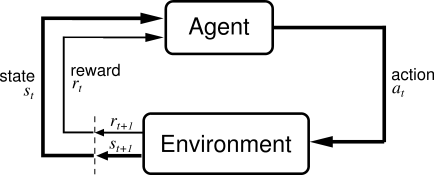
\includegraphics[scale=0.25]{diagram1}
        \end{figure}
        }
        \item{How can we train the agent to pick actions to maximize reward?}
        \item{Goal: Learn parameters $\theta$ to stochastic policy $\pi_\theta(a_t|s_t)$}
        % \item{Objective $\eta$ is $\max{\mathbb{E}\left[\sum_{t=0}^H{\gamma^t r_t}\right]}$}
        \item{Objective $\eta$ is $\max{\mathbb{E}\left[  \gamma^t  \int_t^H{r(t)\mathbf{d}t}  \right]}$}
    \end{itemize}
\end{frame}
\begin{frame}
    \frametitle{Background: ML}
    \begin{itemize}
        \item{Machine Learning Paradigm (using Neural Networks):
        \begin{figure}[p]
            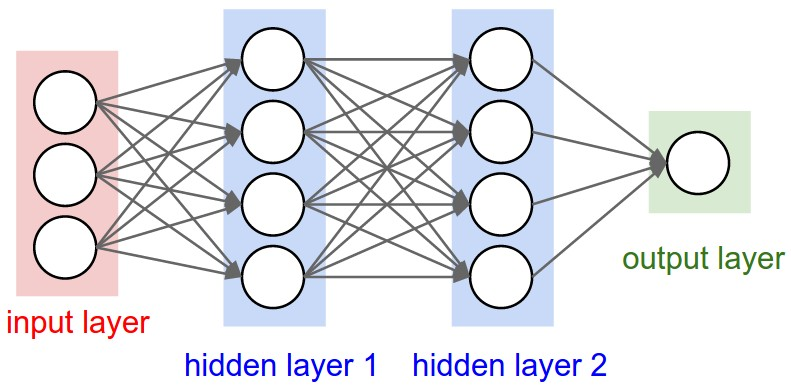
\includegraphics[scale=0.2]{diagram2}
        \end{figure}}
        \item{Goal: make predictions}
        \item{Given many samples of $(x,f(x))$, learn $h_\theta(x)\approx{f(x)}$}
    \end{itemize}
\end{frame}
\begin{frame}
    \frametitle{Current Work}
    \begin{itemize}
        \item{Algorithms are starting to use deep machine learning:}
        \begin{itemize}
            \item{Google DeepMind's Deep-Q-Learning which has learned to play Atari games}
            \item{UC Berkeley's Guided Policy Search which taught a humanoid robot to assemble toy airplanes}
        \end{itemize}
        \item{Different ML Architectures:}
        \begin{itemize}
            \item{Modular Neural Networks}
            \item{Progressive Neural Networks}
            \item{Reccurent Neural Networks}
        \end{itemize}
    \end{itemize}
\end{frame}
\begin{frame}
    \frametitle{What makes Deep RL for Robotics hard?}
    \begin{itemize}
        \item{Lack of large datasets (i.e: poor supervision)}
        \item{Noisy input and can't be sure of outputs}
        \item{Occlusions}
        \item{Running on a real robot is expensive}
        \item{Curse of dimensionality}
        \item{Sparse and time-delayed rewards}
        \item{Exploration vs. Exploitation}
        \item{Continuous control harder than discretized actions}
    \end{itemize}
\end{frame}
\begin{frame}
    \frametitle{Current Tools}
    \begin{itemize}
        \item{OpenAI Gym: Platform for testing general RL algorithms}
        \item{MuJoCo: Efficient simulator used by OpenAI Gym}
        \item{OpenAI RL Lab: implements some common RL algorithms}
        \item{Guided Policy Search: A type of Deep RL algorithm that has a package available online, also uses MuJoCo}
        \item{DeepMind's Lab: 3D first-person games for testing Deep RL algorithms}
    \end{itemize}
    All have elements of robot learning, but don't provide a framework for it % are targeted towards it specifically
\end{frame}
\begin{frame}
    \frametitle{Experimental Design}
    \begin{itemize}
        \item{Collect MuJoCo Robot Models}
        \item{Build an open-source framework with models and other tools}
        \begin{itemize}
            \item{OpenAI MuJoCo Python bindings and Gym}
        \end{itemize}
        \item{Run RL algorithms}
    \end{itemize}
\end{frame}
\begin{frame}
    \frametitle{Data Collection}
    \begin{itemize}
        \item{Task: Peg Insertion with $r=\frac{1}{||x-x^*||}$}%\left( \frac{\|P\|}{2} \middle\| Q \right)$}%$r=\frac{1}{||x-x^*||}$}
        \item{Methods}
        \begin{itemize}
        \item{Random: take a sample from the action space}
        \item{Cross-Entropy Method: sample parameters, evaluate, and reuse best ones}
        \item{Policy Gradient Method: Use trajectory $\langle s, a, r, s' \rangle$ to $\theta_{k+1} \leftarrow \theta_{k} + \alpha\nabla_\theta \eta$}
        \item{Guided Policy Search: uses trajectory optimization to train the neural net based policy}
    \end{itemize}
\end{itemize}
\end{frame}
\begin{frame}
    \frametitle{Graphs (Reward vs Time)}
    \begin{figure}
        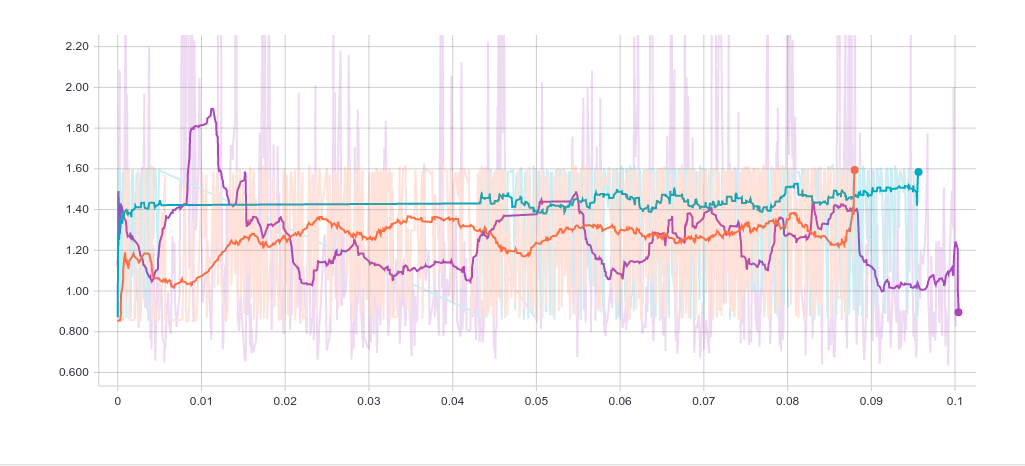
\includegraphics[scale=0.2]{smoothed}
    \end{figure}
    \begin{itemize}
        \item{Collected using TensorFlow's TensorBoard Visualizer, using a $0.6$ smooth}
        \item{Teal line is policy gradient, orange line is cross-entropy, purple is random}
        \item{Random has erratic behavior and inconsistent results as expected}
        \item{Cross entropy is somewhat unstable but leads to more consistent results}
        \item{Policy Gradient seems to have reached a local optimum}
    \end{itemize}
\end{frame}
\begin{frame}
    \frametitle{Discussion and Future Work}
    \begin{itemize}
        \item{Continue to maintain the framework and create documentation}
        \item{Experiment with modular networks}
        \item{Benchmark more deep learning based algorithms}
        \item{Try different tasks and rewards}
    \end{itemize}
\end{frame}
\begin{frame}
    \frametitle{Acknowledgements and References}
    \begin{itemize}
        \item{Thanks to}
        \begin{itemize}
            \item{Mr. Martin Baynes for sponsoring this project}
            \item{Soroush Nasiriany, an undergraduate researcher at UC Berkeley, for feedback on this project}
        \end{itemize}
    \end{itemize}
\end{frame}
\end{document}
